\chapter{Search by Object Location}
\label{ch:object_location}

\todo[inline]{v grafe, na x ovu os dat rank}
\todo[inline]{\% of searched target images up to a given rank}
\todo[inline]{preklesit sipky a rozdelit tie modre konce od seba}


\normalem
\emph{You see a picture in your head. Your friend was standing on the beach, and there was a little sandcastle on the left. The sea behind beautifully reflected the sun, which was setting.}
\ULforem

We can imagine that at that particular moment we were shooting a video of the scenery. However, years later, with a vast set of videos in our collections, it may be impossible to re-watch every one of them to find that particular memory. Not all of us can visualize the memory, but about those who can, we say that they have an excellent visual memory \footnote{\url{https://en.wikipedia.org/wiki/Visual_memory}}. We present a technique that can be used to search in a dataset based on such memories of the scenery.

In this chapter, we elaborate approaches for known-item search task based on the visual description of the image. The input characteristics are that we can recall how the objects looked (i.e., a person had a red hoodie) and their relative location in the image (i.e., top left corner). With that information, we look at the match in the database for a described image. We encapsulate the information in input and refer to it as a \emph{collage}. It means taking images and placing them onto an empty canvas. The placement of the images also carries a piece of information. We show an example of such a collage (query) in figure \ref{fig:query_collage_comparison}. On the left, we can see a cat in the center behind a window. On the right, we can see a possible visualization of such memory. On the grey canvas, we placed a window, which reminded us of the original one. At the center, we added a similarly colored cat.

\begin{figure}
\centering

\begin{subfigure}[t]{0.45\textwidth}
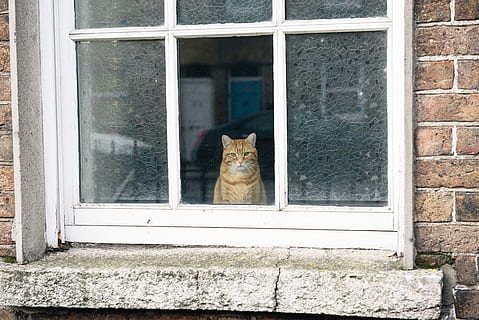
\includegraphics[width=0.9\linewidth]{img/cat_on_window} 
\caption{Query}
\label{fig:searched_scene}
\end{subfigure}
\begin{subfigure}[t]{0.45\textwidth}
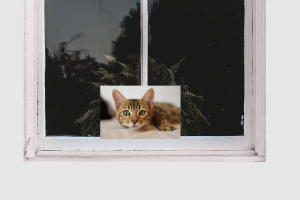
\includegraphics[width=0.9\linewidth]{img/cat_on_window_collage}
\caption{One of the possible collage description for the query}
\label{fig:collage_example}
\end{subfigure}

\caption{Example of searched scene (query) with possible visual description by a collage.}
\label{fig:query_collage_comparison}
\end{figure}

While we were describing the image, we used words for it. However, in this chapter, we do not focus on the search based on the verbal description of the objects. However, it is one of the possible alternatives to handling the problem. Supporting verbal descriptions often require extensively annotated data to use to train neural networks, and even though the advancements in the research area, it still has a limited ability for extensively described characteristics. Our approach aims to avoid these limitations of vocabulary size. We believe that visually we can capture more diversity. Words often omit more specific information about the look or are hard to obtain by annotation systems, since the annotation tool may have never seen such combination before. For example, a single word for a human may represent a visually wide range of possibilities, based on clothes, age, and other attributes. We aim to avoid this bottleneck, and we proceed with the search based visual similarities.


In this chapter we utilise approaches for solving known-item search task based on \emph{collage}. Collage $C$ is a (unordered) set of $k$ pictures $C = \{\text{collage\_image}_i\} \text{for}\, i \in \{1, 2, \dots, k\} $.  Each $collage\_image_i$ contains two characteristics: image (i.e., visual description) and spatial information (location). To avoid any scaling and resolution issues, we represent location by a relative offset from the left, top, bottom and right. Therefore, all attributes of spatial information are in range $[0,1]$

This chapter will present three approaches incorporating pre-trained neural networks. To learn more about the networks, head back to chapter \ref{ss:pretrained_models}. We start by a short description of user-program interaction to understand the origin of the queries we evaluate. The chapter invites the ideas with their evaluation. We test a different set of hyperparameters and investigating their effect on the performance of the system. More information about the dataset is provided in section \ref{s:dataset}. To learn more about the user-interface, check the documentation in chapter \ref{ch:user_guide}. 


\section{User-program interaction}

The query is a \emph{collage} of one or multiple images. Each image also includes its relative position in the canvas.

We provide a user with a canvas where she can place, move, and resize the images in the \emph{collage}. Interactively, the set of results is showed (the most similar results). The user can then alternate the query for a new search, or to investigate the displayed results. Figure \ref{fig:query_collage_comparison} shows an example of the query -- the collage of two images (window and cat). 

\section{Framework overview}

In the rest of the chapter, we present different approaches to this task, and we test different settings to obtain the best set of hyperparameters. In figure \ref{fig:processing_pipeline}, we can see an overview of the system. The top path is a processing path for the items in the database. The features are precomputed (offline) for all images in the database. We call a \emph{record} an image with its features. Each of the features may also be linked with additional information. There is one record per input image, but each record may contain multiple feature vectors describing it.

Similarly, for a given collage, we extract features by using the same model as for the database extraction. We do that for each of the images in the collage. Since we only need to annotate a couple of images, this can be done online on CPU for most neural networks. In this phase, we have an annotated dataset and extracted features from query images. Next, if the records contain multiple feature vectors, we may filter them to decrease the number of vectors we will compare. We call this process \emph{Relevant Features Extraction}. Next, based on the features from the database and the features from the collage, we compute their distances. For each query image, we compute the distance to each record in the database. This step creates a ranking of the database records for each input image in the collage. The last step is to merge these rankings. In the example image, a final merged ranking is computed based on the average distance for all query images.

We tune several factors in the described pipeline. In the following text, each step is described individually. Although, since they create a system as a whole, we evaluate them in the full environment, but always focusing on the particular part we test. For the next sections, we progressively build the pipeline while describing the particular approaches we used. We start with feature extraction strategies, and then we continue with the next steps, which are independent of feature extraction.

\section{Features extraction strategies}

In the following section, we present three feature extraction techniques. The feature extraction technique defines how we extract features for our dataset as well as for our queries. These obtained features will be later compared against each other in a ranking mechanism. We kick off with the baseline, where we do not use the location of the objects in the collage. Then we move on to an approach, which splits the image into regions and compares only to the regions related to the object query. Our last method is experimental, and it involves storing a higher-dimensional feature vector. This approach performs no strict pre-cutting. Instead, it works with the last convolutional block from the neural network.

\begin{figure}[p!]
    \centering
    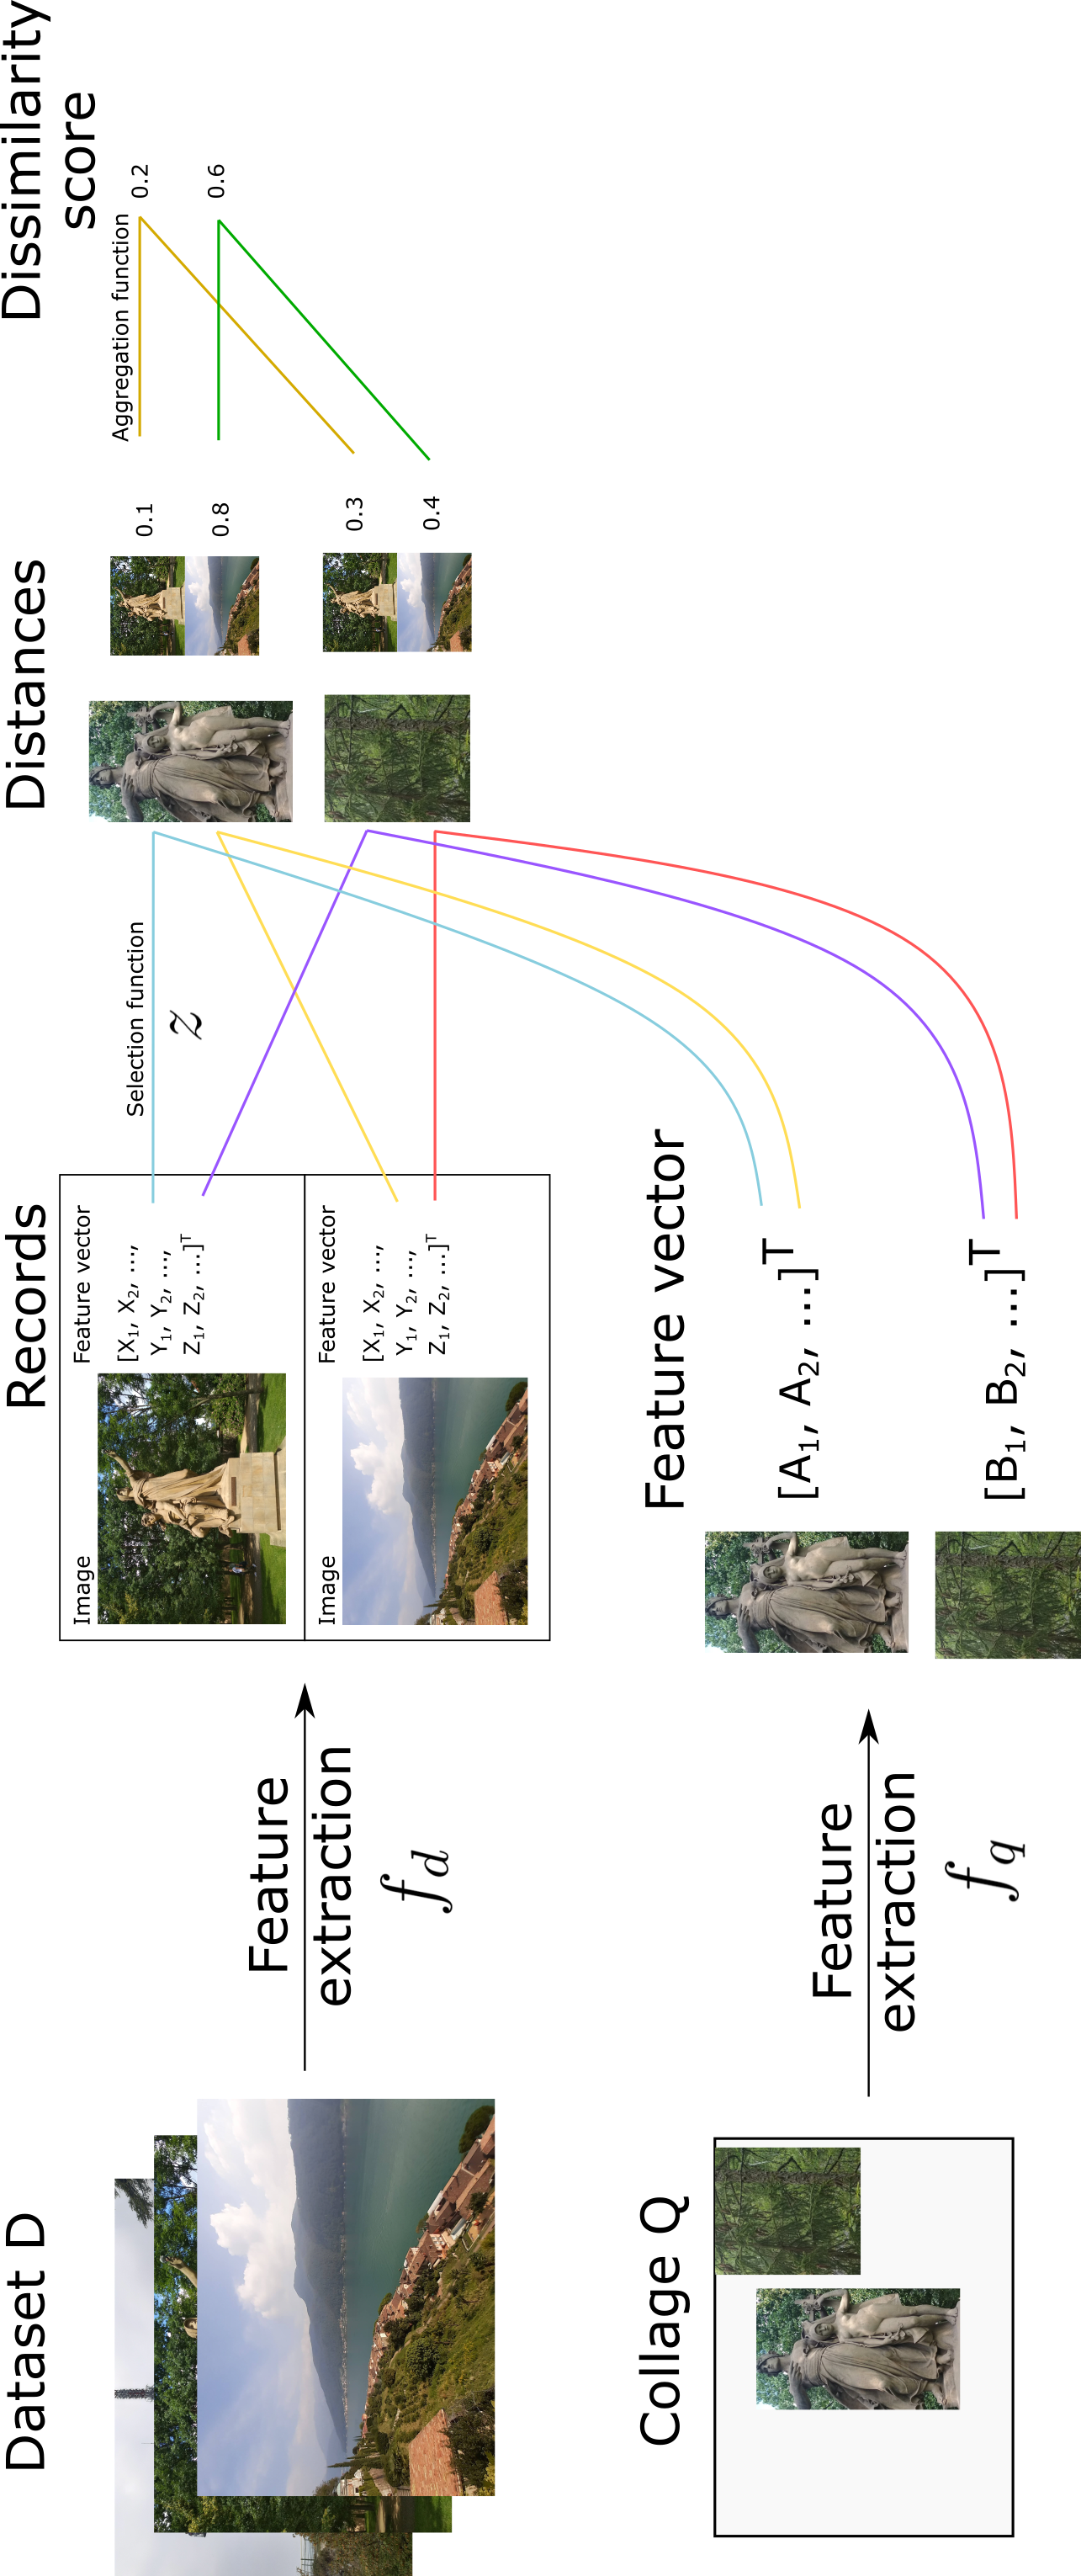
\includegraphics[scale=0.9]{img/features_pipeline.png}
    \caption{Overview of processing pipeline}
    \label{fig:processing_pipeline}
\end{figure}

\subsection{Baseline -- Image representation}

Firstly, we developed a simple approach, which ignores the information about the position of the images in the collage. We set this approach as our baseline to see how much we improved a simple technique like this by adding more complexity. For each image in the dataset, we compute one feature vector by feeding it to the pre-trained convolutional neural network. The images in the dataset are rescaled (without preserving ratio) to fit the network's input dimensions (224x224).

In figure \ref{fig:mobilenet_whole_image_example}, used for the explanation of the graphs, we show the performance on the annotated set of collages. We present the results on the MobileNetV2. We use MobileNetV2 due to its low computability needs and therefore offering quick annotations. It is widely used in the task, where we expect online or near online evaluation. We included a short description of the Related Work (section \ref{ss:pretrained_models}).

\begin{figure}
\centering
\begin{boxedverbatim}
Database:
    - image: 1 feature vector
Query:
    - query_image: 1 feature vector
    - compared to: each feature vector in the dataset
\end{boxedverbatim}
\caption{Overview of the Image representation approach}
\end{figure}

\subsection{Splitting an Image into Regions}

Our goal in the next presented approach is to use also the information about the objects' location. Our dataset contains many different images, with objects in different positions. Although, as we have seen in the previous section, comparison to the whole image worked well. Here we propose to include higher granularity and to split the image into multiple regions. That way, we can compare the query images only to the region, which is related (for example, if the tree is placed in the bottom right corner, we would compare only to the region from the bottom right corner). If we cut each image to the same regions, we will also be able to speed up the processing.

We define cutting into regions. Each record contains one image, which is visually divided into  $N \times M$ regions. Then for each region, we compute a feature vector via a pre-trained model. When the query comes, we will compare the query image only to the regions from the record, which overlap.

\begin{figure}
\centering
\begin{boxedverbatim}
Database:
    - image:
        - multiple regions:
            - region's coordinates
            - feature vector
Query:
    - query_images: feature vectors
    - compared to: only to related crops from each image
\end{boxedverbatim}
\caption{Overview of the Regions' approach}
\end{figure}

\subsubsection{Regions Shape}

To use transfer learning for conventional CNN and avoid additional skewing in resizing, we limit the regions to the shape of squares. Since this input size of the square is one of the parameters, we aim to use the squares size the same as the size of the input of the network. Keeping square regions helps us avoid unnecessary scaling, which may be introduced when the length of the square's side does not match with the input for the network.

A second limitation we create is for the regions to cover the image entirely. Since we now know we need square regions that cover a full image, there might be no way to cut an image into the regions without overlapping. Therefore, we create enough regions to cover the image entirely and split the excess between the regions. This excess is evenly distributed over the regions, creating equal overlaps. We split based on the predefined number of regions since the number of regions results in the complexity's multiplicative coefficient.

Allowing overlaps plays another role in this technique. With the rigid frame without overlapping, it could happen that they would split an object into two parts. With overlaps, we know that some part is shared between both regions.

Our fixed parameters are input shape width $s$ and the number of regions we want to use $N \times M$ and image size $h, w$. We solve the task of choosing regions splits for one axis; the second is done equivalently. We know that the last region has to end with the edge of the image. Therefore the starting coordinate of the last region is $h - s$. We then split the remaining "space" over axis over $N-1$ regions equally. We call this distance $step$ since it says the distance between the regions. The starting coordinate $r_i$ of the $i$-th region in a given axis is:

\begin{align*}
step_h = (h - s) / (N - 1) \\
r_i = {i \, step_h\,\text{for}\,i \in \{0, 1, 2, \dots, N - 1\}}
\end{align*}

With the condition on full coverage of the image (i.e., \(s N >= \text{h}\), and for $M$ respectively), we obtain full coverage of the image by the regions. Overlaps are evenly distributed over both axes. Although, with bigger sized regions, overlaps may occur between more than two regions. For example, if we split an image with width 180 into three regions with a width of 96 pixels, some areas of the image will be included in all three regions. This happens, when the $step \leq 2 s$.

We evaluate the performance of the same network using a different number of regions. This experiment is shown in the figure \ref{fig:different_number_regions}. Even though the number of regions was almost doubled (from 8 to 15), we only saw a slight improvement in performance. In the figure \ref{fig:different_region_size} we show the effect of the regions size. We see that the best performing model worked with $2\times4$ regions with the input size of $128\times128$. For this particular setup, it was able to rank 90\% of the collages in the 8\% of the database.

\begin{figure}
\centering
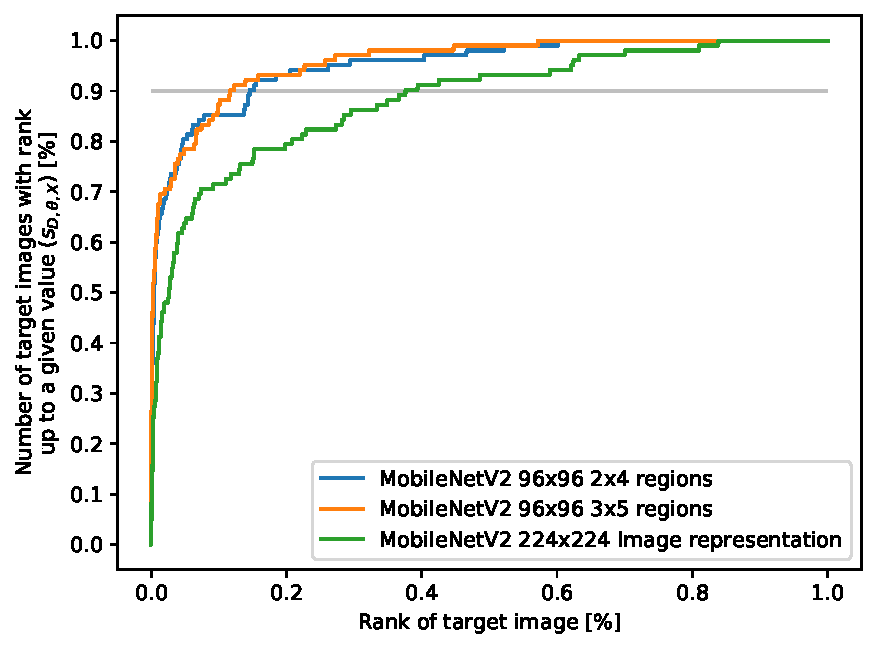
\includegraphics[width=0.8\linewidth]{graphs/0c36458e4a7754f349e4dd02e823acc5f192f0aaa42647313045530525f3db19.pdf}
\caption{An experiment comparing the effect of the changing number of regions.}
\label{fig:different_number_regions}
\end{figure}

\begin{figure}
\centering
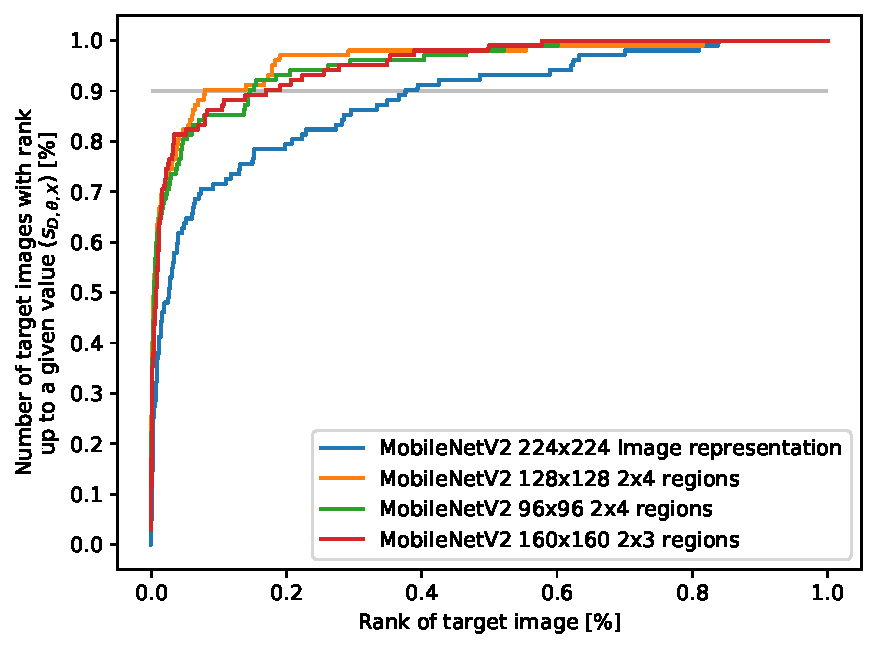
\includegraphics[width=0.8\linewidth]{graphs/901175c0015f71987720d10953133afa566d88a09a6d7182a074859ff4e8409e.pdf}
\caption{An experiment comparing the effect of the changing regions size.}
\label{fig:different_region_size}
\end{figure}


\subsubsection{Choice of regions}

Previously, we defined a cutting into the regions for each item in the dataset. Now we select the regions, which are compared to the query image. We could compare with all that overlap with the location of the query image. Although there might be many of those. For example, let us assume we have a query image that covers two-thirds of the canvas. In such a case, it probably overlaps almost all or at least most of the regions. Comparing the features with all of them is less effective than choosing only some of them.

Given one incoming query image with its position and shape, we propose several methods for choosing the "selected" regions. We visualize the problem in the figure \ref{fig:fish_with_grid}. The query would be an image of the fish placed within the red boundary. We mark all overlapped regions with a green line. The region with the highest "coverage" is the blue one.

One approach is to choose the region which overlaps with the query the most (in the example, the blue one). To do that, we compute Intersection over Union (\ref{fig:intersection_over_union}) for each of the regions. This metric tells us which of the regions are more covered by the query and which less.

\emph{Intersection over Union} (also known as Jaccard index\footnote{\href{https://en.wikipedia.org/wiki/Jaccard_index}{https://en.wikipedia.org/wiki/Jaccard\_index}}) measures similarity between two sets. We use it as a metric to express how much two regions (i.e., two rectangles) overlap. 

The definition of the Intersection over Union is following:
$$
    J(A, B) = 
    \begin{cases}
      1, & \text{if\ A and B are empty} \\
      \frac{|A \cap B|}{|A \cup B|}, & \text{otherwise}
    \end{cases}
$$

In our case, the $|A \cap B|$ represents the area that belongs to both regions. The  $|A \cup B|$ represents the area covered by the union of both regions. A visual representation of the formula is displayed in the Figure \ref{fig:intersection_over_union}.

\begin{figure}
    \centering
	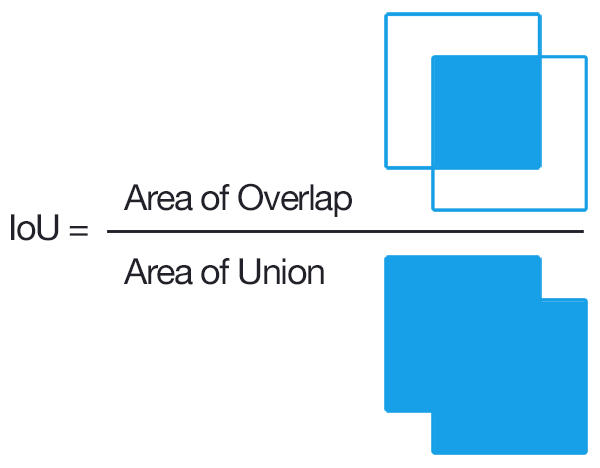
\includegraphics[width=0.3\linewidth]{img/Intersection_over_Union_-_visual_equation.png}
	\caption{Intersection over Union between regions. Source: Wikipedia, CC BY-SA 4.0}
	\label{fig:intersection_over_union}
\end{figure}

With the selected regions, we compute the distance between the query image and each of the regions. For each record from the dataset, we select only one region, which has the lowest distance to the query.
We present an experiment, where we took all intercepted regions (green regions in the example), only the region with the highest IoU (blue region in the example), or equivalently first 2 with the highest IoU or first three regions. The results of the experiment are shown in figure \ref{fig:crop_limitation}. In the results, we see no significant improvement in any of the provided choices. Although, the selection of only the region with the highest overlap gives us the least computable heavy approach.

\begin{figure}
\centering
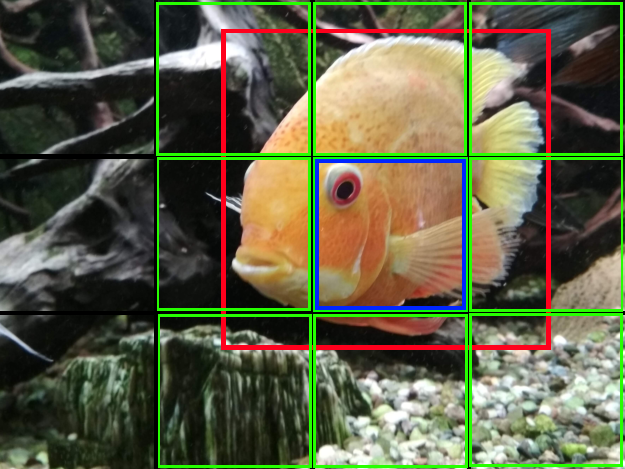
\includegraphics[width=0.6\textwidth]{img/fish_grid_regions}
\caption{Example of choosing the corresponding regions. Red: query position; Green: all intercepted regions; Blue: region with highest IoU.}
\label{fig:fish_with_grid}
\end{figure}


\begin{figure}
\centering
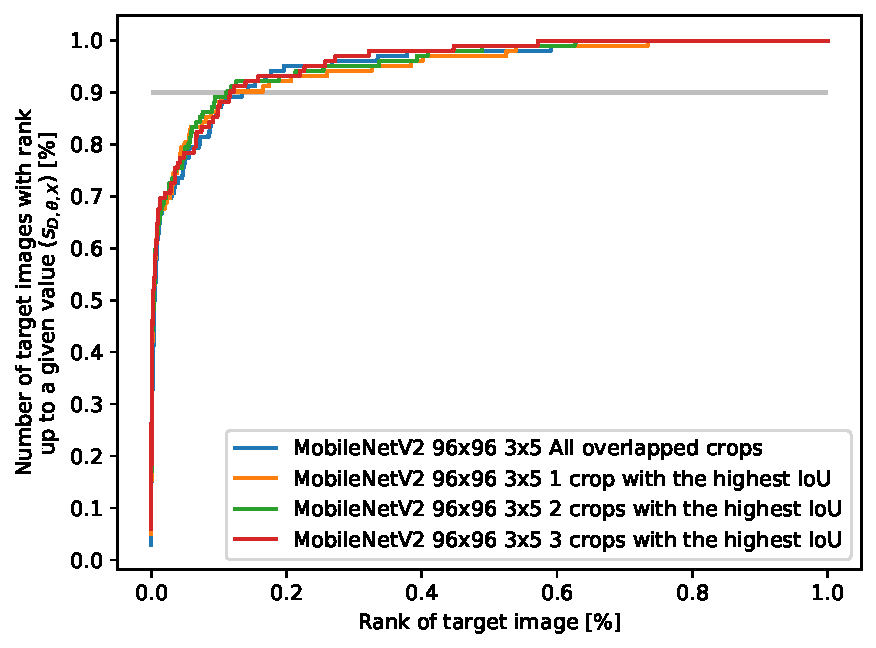
\includegraphics[width=0.8\linewidth]{graphs/5c4a781f8e6f3eac93db2083bde3963c06582a92a8141411bf29e41251a98e75.pdf}
\caption{Performance of the system based on different number of chosen crops}
\label{fig:crop_limitation}
\end{figure}

\subsection{Using the whole last convolution block}

In the previous section, we worked with cutting into fixed regions. Although we reached a good performing model, we can see it has a shortcoming. The cutting into regions does not adapt to the size of the input query. Let us retake a look at the fish in figure \ref{fig:fish_with_grid}. We can see that fish covers circa two-thirds of the image, but the regions cover only one-twelfth. The regions do not offer any adaptation to the size of the query. It means that big query images are processed in the same way as small.

We investigated the structure of the CNNs, and we propose an approach. We use the last convolutional block as our feature vector. Since the CNNs consist of several convolution blocks before pooling, we extract the information from the last one. Before, we stripped the fully connected layer to obtain the feature vector after pooling. Now, we strip global pooling to retrieve only the convolutional block. These blocks usually end with a ReLu activation function.

Why is it important? The Global Pooling reduces the feature vector from produced by the convolution block from  $\mathbb{R}^{n\times m \times c}$ to  $\mathbb{R}^{c}$ (the same space was used for features in regions' approach). Due to the convolutional neural network principle, we assume we could retrieve more information by working with the layer before pooling. This layer does not only contain the final feature vector but contains additional spatial information.

We refer to the last layer we are interested -- convolutional block with ReLu as \emph{antepenultimate} (i.e., last but two). 

\begin{figure}
\centering
\begin{boxedverbatim}
Database:
    - image:
        - feature vector (last convolution block):
Query:
    - query_images: global average pooling over feature vectors
    - compared to: pooling over selected region
\end{boxedverbatim}
\caption{Overview of the Approach with last convolution block}
\end{figure}


\subsubsection{Choosing a region of interest in the layer}

Layer before pooling on which we focus (antepenultimate) is the last convolution block. Therefore, it produces features from space $\mathbb{R}^{n\times m \times c}$, where $n, m, c$ is the shape of the convolution block. The first two dimensions contain spatial information, which is propagated from the previous layers. The third represents the channels (i.e., features).

To obtain only a part of this layer, we are interested in (i.e., our query was placed in that specific region); we need to take only a subset over the first two dimensions. For a query defined by region $R_i = (y, x, h, w)$ and a hidden layer $L_i$ with dimensions $(H, W, C)$ we consider select following subset of the layer: $L_i[y * H: (y+h) * H][x*W, (x + w) * W][:]$. We use a notation that, for a given dimension, $:$ represents a half-open interval. If there are no limits, then it represents taking the vector fully in a given dimension.

Both MobileNetV2 and Resnet50V2 end with a convolution block with dimensions $(7,7,C)$, where $C = 1280$ for MobileNetV2 and $C = 2048$ for Resnet50V2. Previously mentioned selection of interesting regions may result in empty selection. For example, when the query image covers only one-tenth of the image in both dimensions. The rounding may result in an empty interval. We solve by adding one to the dimension, whenever it would be empty.

Now, we selected a subset of the last convolutional block. The original network follows with \verb+GlobalAveragePooling2D+. We perform the same operation on the selected subset. This way, we again obtain the feature vector from $\mathbb{R}^c$ for each record.

Compared to the previous approaches, we aim to avoid strict cutting and provide more flexibility. On the other hand, this approach requires more memory since we store 49 feature vectors per vector ($7\times7$). We present the results in figure \ref{fig:antepenultimate}. Due to its memory limitation, we downsized the dataset to one-tenth. We randomly sampled the images from the dataset. We provide a baseline on this smaller dataset. We can see an improvement compared to the baseline. We were able to implement spatial information of the query successfully. However, the performance is worse compared to one of our region's techniques. We assume that this is caused by the fact that running a network 15 times can extract more information than running it only once.

\begin{figure}
    \centering
    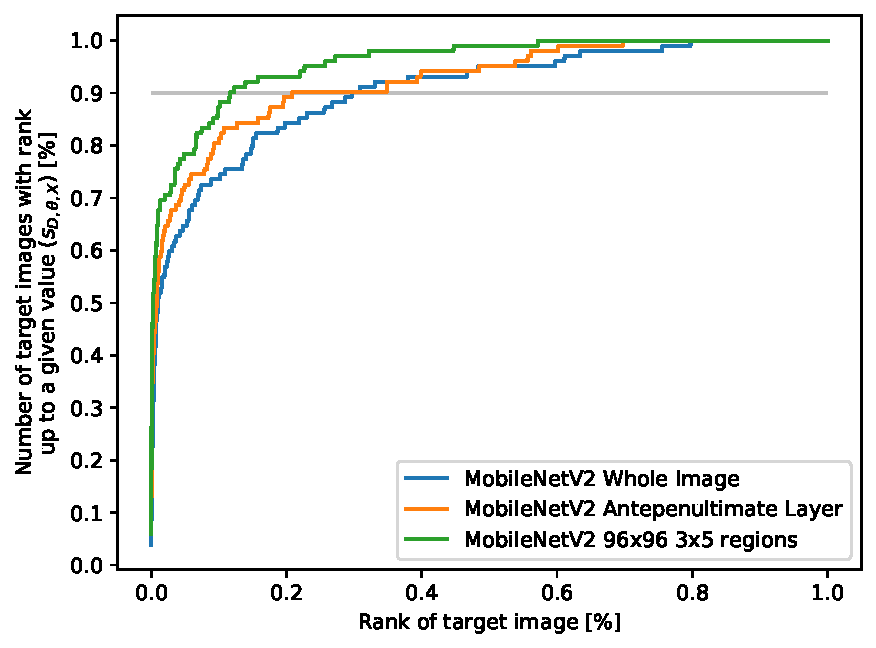
\includegraphics[width=0.8\linewidth]{graphs/adaf8d435bb40406f9ce40654ec396e04453ab76cf0776d2a87d385055d5424f.pdf}
    \caption{Comparison of baseline, regions and aproach using the antepenultimate layer.}
    \label{fig:antepenultimate}
\end{figure}

\section{Ranking}

Let us remind an overview from figure \ref{fig:processing_pipeline}. In the previous sections, we have seen two approaches presented for feature extraction. The first one was based on the regions, the second one based on the antepenultimate layer from CNN. Now we will continue in the second part of the pipeline, extracting distances and ranking the records in the database. We continue to work with our so far best-performing model -- MobileNetV2 spitted into 2x4 regions with the input size 128x128.

In the previous sections, we talked about obtaining feature vectors for the items in the database while selecting only relevant regions. In this section, we take a closer look at further processing these obtained feature vectors.

We extract features for query images the same way (using the same model) for the items in the dataset. Then, we compute the distance between the query image and the items in the dataset for each query image.

Based on these distances, we order the results, starting from the smallest distance. This distance acts as an inverse for the similarity. More similar the results are, the smaller is the distance.

In figure \ref{fig:regions_distances}, we show a comparison between three different distance measures we compared. We see a superior performance of the cosine distance over Euclidean and Manhattan distance. Since we work with a high dimensional space (in case of MobileNetV2, it produces 1280 dimensions after pooling), the Euclidean distance suffers from the curse of the dimensionality\footnote{\url{https://en.wikipedia.org/wiki/Curse\_of\_dimensionality\#Distance\_functions}}. 

\begin{figure}
    \centering
    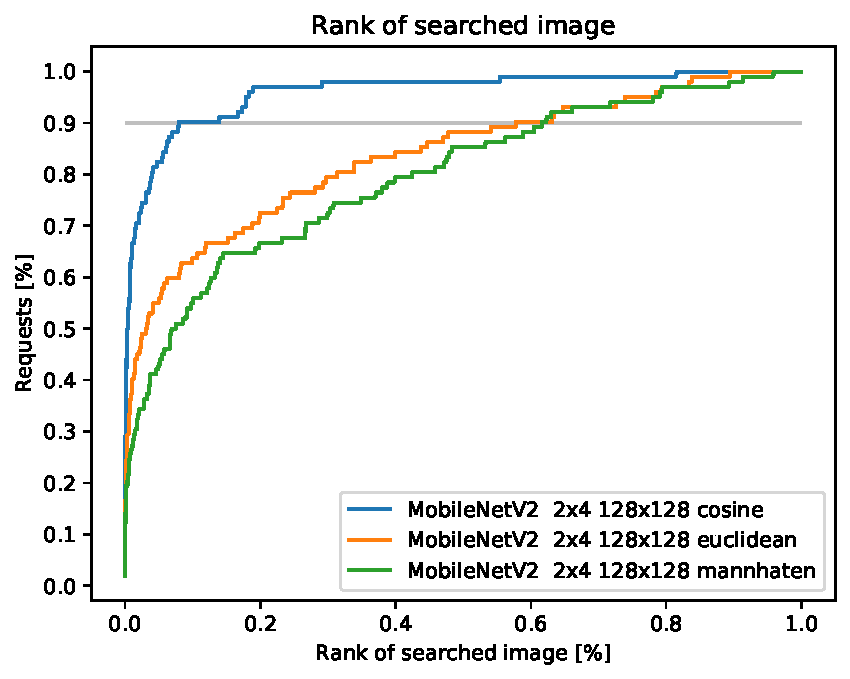
\includegraphics[width=0.8\linewidth]{graphs/3aab502ea602a9f49afaa0a0d998cf226a0a67b9efcaa655d2ddf5063eeabe47.pdf}
    \caption{Comparison of the performance based on the chosen distance function.}
    \label{fig:regions_distances}
\end{figure}

\section{Multiple objects in the scene}

We already discussed techniques for feature extraction and distance. We produced the ranking of the dataset for each query image. In this section, we solve a question of how to merge these rankings from multiple query images to obtain one final ranking, which is presented to the user.

For our task, we do not assign any weights to the input query images. We neither work with the order of their placement. A collage is an unordered set of images with their location. In this section, we assume we already have the ranks per query image. Our goal is to merge them and produce one ranking.

We define ranking $R$ as a set of distances between the query image $q$ and database item $i$. We look for a function $r: R^n \rightarrow R$, which merges multiple rankings into one final ranking.

We test three such functions, $min(\cdot)$, $mean(\cdot)$ and $max(\cdot)$.  For a database image, we compute the distance as a given function from the distances to the query images. Afterward, we rank the database images based on their distances. 

A comparison of these functions for MobileNetV2 can be seen in figure \ref{fig:ranking_funcs}. The $min(\cdot)$ has the advantage of "forgiving" if some of the images provided in the collage were unrelated. The $max(\cdot)$, on the other hand, ranks the images based on the worst match. As our results show, it best performs $mean(\cdot)$, as it assigns the importance to each image from the collage equally.

\begin{figure}
\centering
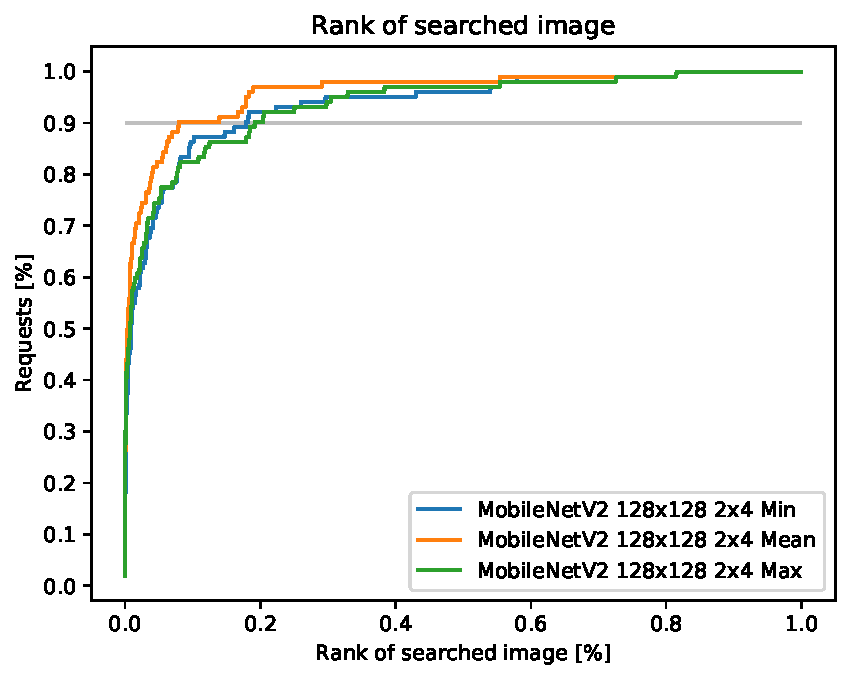
\includegraphics[width=0.8\linewidth]{graphs/70c56dc52be92e048f57b9bdfb35ddce2be41fd2454ae360588da2e387b09de5.pdf}
\caption{Performance of the system based on different ranking function}
\label{fig:ranking_funcs}
\end{figure}

\section{Padding}

We talked about the importance of the square input in the Regions section. During the development, we also explored preprocessing techniques for query images.

Our input to the network is a square. From the user's point of view, we support rectangles. The option to create non-square queries comes handy when the user wants to include, for example, a picture of a person standing, or kayak. A question arises, what is the best way to edit the image to fulfill the square requirement. We test three techniques: rescale, black padding, and white padding. The disadvantage of the rescale is that it distorts the proportions. If the person in the query image is in a tall and narrow box, the distortion will cause it to appear more full and shorter. The distortion becomes stronger with an increasing imbalance between the box dimensions. 

Our question is if it is better to distort the image or provide the image with padding to fill the square shape. For almost square images, the padding covers only a small portion of the image. For images with a significant imbalance in the dimensions, it includes much space with no useful information for the network. A second question we ask is if the color of the padding results in different performance.

The results are shown in figure \ref{fig:padding}. We can see that a rescaling achieved the best performance. A small improvement is achieved by using white padding instead of black. Since the results show favor in rescale, we use it for all other experiments.

\begin{figure}
    \centering
    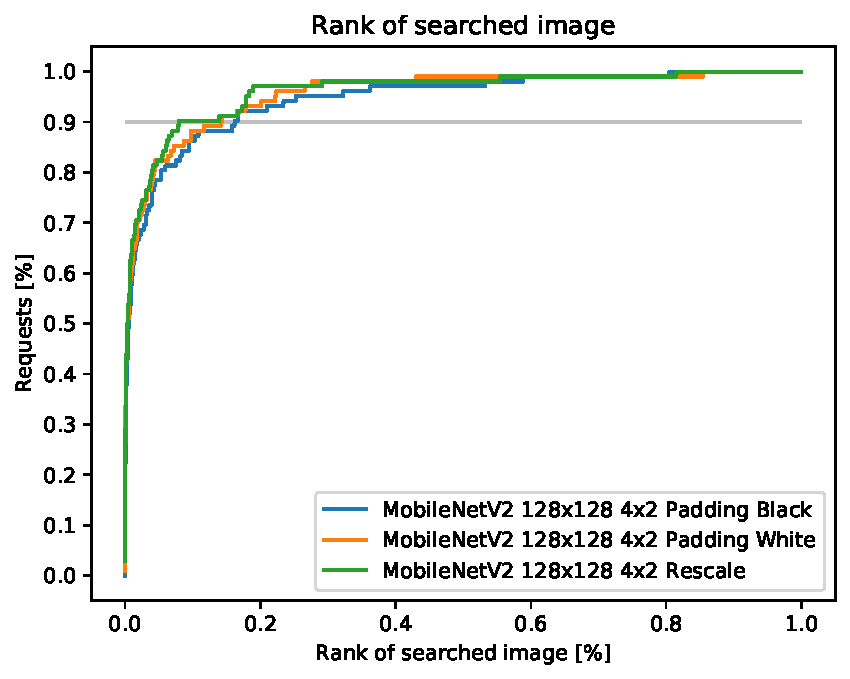
\includegraphics[width=0.8\linewidth]{graphs/bf57efafbbbc7b5a1744054d87d4ecfa381c9eaf2459186904190d97bcb99a81.pdf}
    \caption{Comparison of different padding method for images in the query.}
    \label{fig:padding}
\end{figure}

\section{Dimensionality reduction}

In the previous sections, we evaluated several hyperparameters of the system to achieve the best performance. In this section, we take a look at reducing the dimensionality of the extracted features. Dimensionality reduction could help us to scale our approaches to even bigger datasets and to decrease the query response time.

The extracted features from the neural networks are from high-dimensional space (for MobileNetV2, it is 1280 features, for Resnet50 it is 2048 features). The dimensionality reduction can also have a positive effect on reducing noise if present in the feature vector. We test the performance of the system based on the number of features used. We use the Principal Component Analysis for dimensionality reduction. The results are shown in figure \ref{fig:pca}. From the results, we can have several interesting observations. Even with as low as eight components (8 features), we can obtain performance as the original Image representation baseline. With the increasing number of components, the system performs better. With 512 components, it even performed slightly better as the original data. For our purposes, we think that selecting 128 components offer the best performance-cost ratio. With the need for smaller feature vectors, we would select at minimum 64.

\begin{figure}
    \centering
    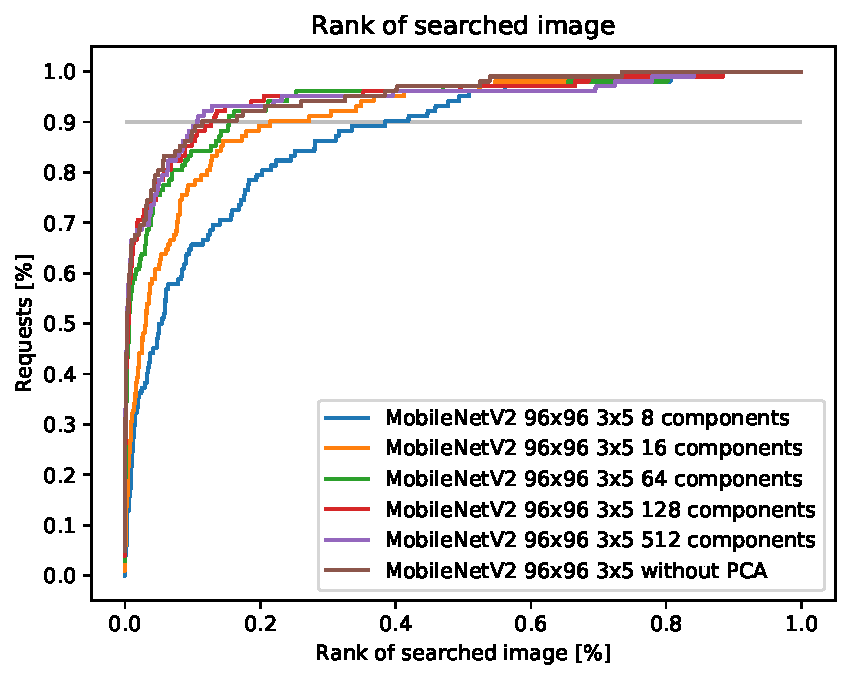
\includegraphics[width=0.8\linewidth]{graphs/6fbd4f70810e1f63f400ef601c1cdba0fd1635749810aa2347a4ff26e6fccf47.pdf}
    \caption{Effect of PCA on the performance of the system}
    \label{fig:pca}
\end{figure}

\section{Neural network selection}

In the previous experiments, we always used MobileNetV2 as our feature extraction model. Thanks to that, we were able to retrieve the best set of hyperparameters for this KIS task. As our last experiment in this chapter, we evaluate the effect of the model on the framework's performance.

In figure \ref{fig:networks}, we present a comparison between the three models. We used two different instances of the ResNet, Resnet50, and Resnet50V2. Networks widely available pre-trained are usually trained on the ImageNet challenge. The task in the challenge is to classify into 1000 classes. In this manner was trained MobileNetV2 as well as Resnet50V2 we used. We present the Resnet50 as model pre-trained on more than eleven thousand classes. We aim to support the claim experimentally that network trained on more classes can achieve a better performance level. In the experiment, we can see that both ResNets work better than MobileNetV2. At the same time, we can see that ResNet trained on more classes performed significantly better in the beginning. Although, we have to note that Resnet50V2 was more successfully solving the rest of the queries.

The downside of using a ResNet50 trained on eleven thousands of classes compared to MobileNetV2 is slower evaluation and availability. Since this is not the challenge, the researchers focus on most, the set of pre-trained neural network for this task is smaller. Also, used Resnet50 is only pre-trained with the input shape 224x224. To use it for the regions, we introduced upscaling for the network input. Even though these difficulties, it proved itself as the best choice out of the compared alternatives.

\begin{figure}
    \centering
    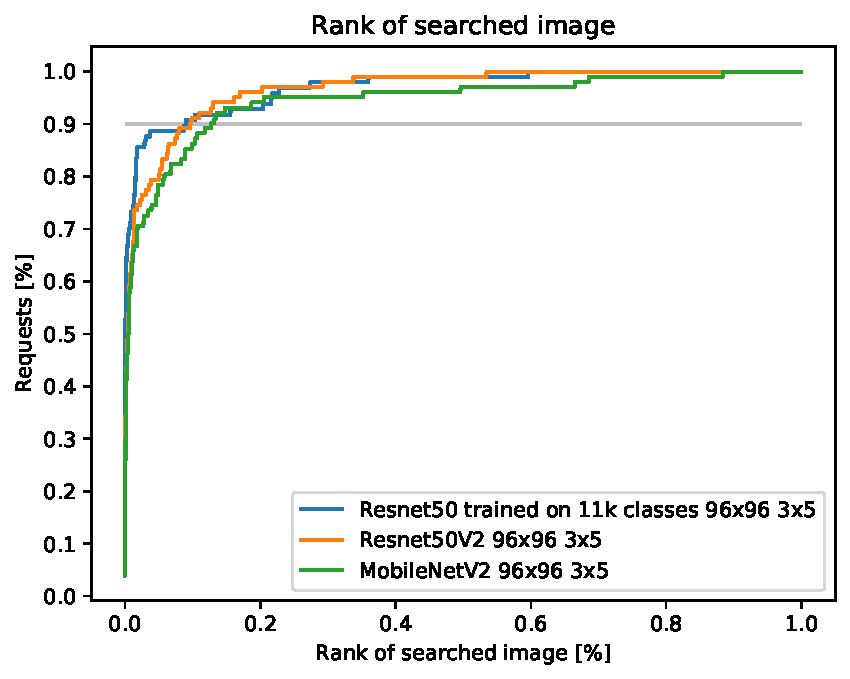
\includegraphics[width=0.8\linewidth]{graphs/2536f6c96149dea24dae84dbf52f760d7d58b0dffa7d660656e1784d9dca277f.pdf}
    \caption{Comparison of the performance based on different feature extraction models.}
    \label{fig:networks}
\end{figure}

\section{Overview of the achieved results}

In this chapter, we tested several hyperparameters for this task. We experimentally proved their validity. The best performing approach was cutting into regions. The setting of \emph{2x4 regions 128x128}, as well \emph{3x5 regions 96x96} performed both well. We found out that the number of selected crops does not have a significant role in improving the searched image's rank. For the distance function, we chose \emph{cosine distance} since it performed significantly better than the others. To merge the rankings, we continue with the \emph{average}. For the padding selection, it emerged from the experiment that \emph{rescale} worked the best. The next hyperparameter, we obtained, is that dimensionality reduction into \emph{128} (ten times smaller than original ones) has almost no effect on the system's performance. From the tested networks, \emph{Resnet50} trained on eleven thousands of classes performed the best.
